\chapter{Manual d'usuari}
\label{cha:userguide}

\section{Casa de l'usuari}
\label{sec:home}
Per accedir la casa del usuari es pot anar accedint mitjançant el logo de ''Ichnaea'' del menú situat a l'esquerra del menú.

\begin{figure}[h!]
  \centering
  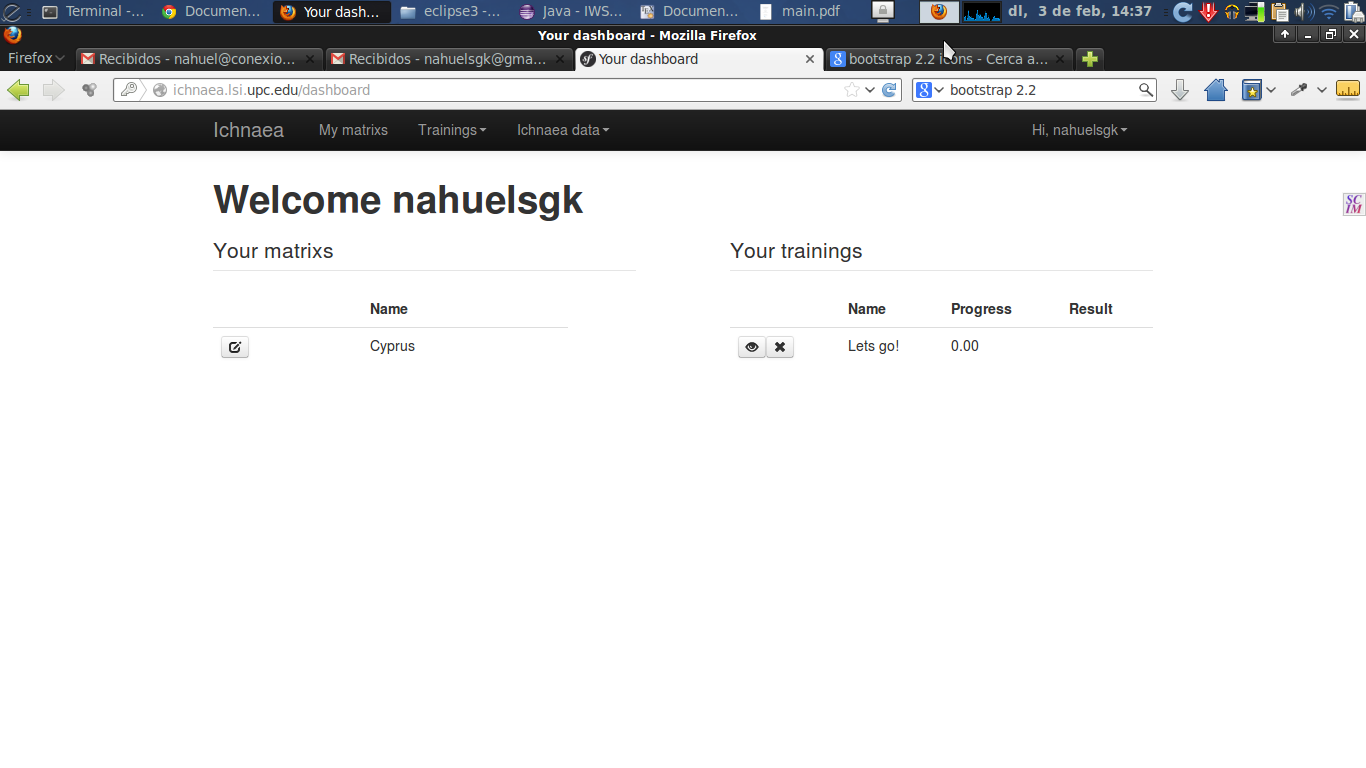
\includegraphics[scale=0.4]{img/userguide/dashboard.png}
  \caption{Casa de l'usuari}
  \label{fig:placement}
\end{figure}
A continuaci\'{o} descriurem cadascuna de les parts.

\subsection{Llistat dels meus entrenaments pendents}
Al llistat superior pots veure els entrenaments que has creat i que estan pendents de finalitzar, on: 
\begin{itemize}
\item Nom del entrenament.
\item Nom de la matriu entrenada com a enllaç per veure la matriu.
\item Descripci\'{o} del entrenament.
\item Origen: Paràmetre de creació seleccionat per l'entrenament. Actualment solament es guarda el valor pero Ichnaea no esta desenvolupat encara per executar un entrenament amb aquest paràmetre.
\item Data de creaci\'{o} de l'entrenament.
\item Nom de l'usuari que la creat(que sempre serà l'usuari registrat).
\item Progr\'{e}s: actualment Ichnaea no retorna estat del proces. Solament ens diu si ha acabat o no. Per tant els \'{u}nics valors son 0.00 i 1.00.
\item Status. Els possibles status son ''pending''(no s'ha pogut enviar),''sent''(s'ha enviat a la cua). Els entrenaments finalitzats es poden consultar a ''Els meus entrenaments''(mirar \ref{subsec:myTrainings}).
\item Error: en cas que hi hagues algun error en el entrenament desde Ichnaea, sortiria un breu descripcio.(Mirar \ref{subsec:trainingerrorsIchnaea})
\item Operacions
 \begin{itemize}
 \item \iconeyeopen es per anar a la pantalla de visualització de l'entrenament.
 \end{itemize}
\end{itemize}

\subsection{Llistat de les meves prediccions pendents}
Al llistat inferior pots veure les prediccions que has creat i que estan pendents de finalitzar, on: 
\begin{itemize}
\item Nom de la predicció.
\item Nom de la matriu entrenada com a enllaç per veure la matriu.
\item Descripci\'{o} del entrenament que s'esta usant en la predicció.
\item Origen: Paràmetre de creació seleccionat per l'entrenament. Actualment solament es guarda el valor pero Ichnaea no esta desenvolupat encara per executar una entrenament amb aquest paràmetre.
\item Data de creaci\'{o} de la predicció.
\item Nom de l'usuari que la creat(que sempre serà l'usuari registrat).
\item Status. Els possibles status son ''pending''(no s'ha pogut enviar),''sent''(s'ha enviat a la cua). Els entrenaments finalitzats es poden consultar a ''Els meus entrenaments''(mirar \ref{subsec:myPrediccions}).
\item Error: en cas que hi hagues algun error en el entrenament desde Ichnaea, sortiria un breu descripcio.(Mirar \ref{subsec:trainingerrorsIchnaea})
\item Operacions
 \begin{itemize}
 \item \iconeyeopen es per anar a la pantalla de visualització de l'entrenament.
 \end{itemize}
\end{itemize}

\subsection{Els meus entrenaments}
\label{subsec:myTrainings}
Per accedir als teus entrenaments, ves al menu ''Trainings >> My trainings''.
\begin{figure}[h!]
  \centering
  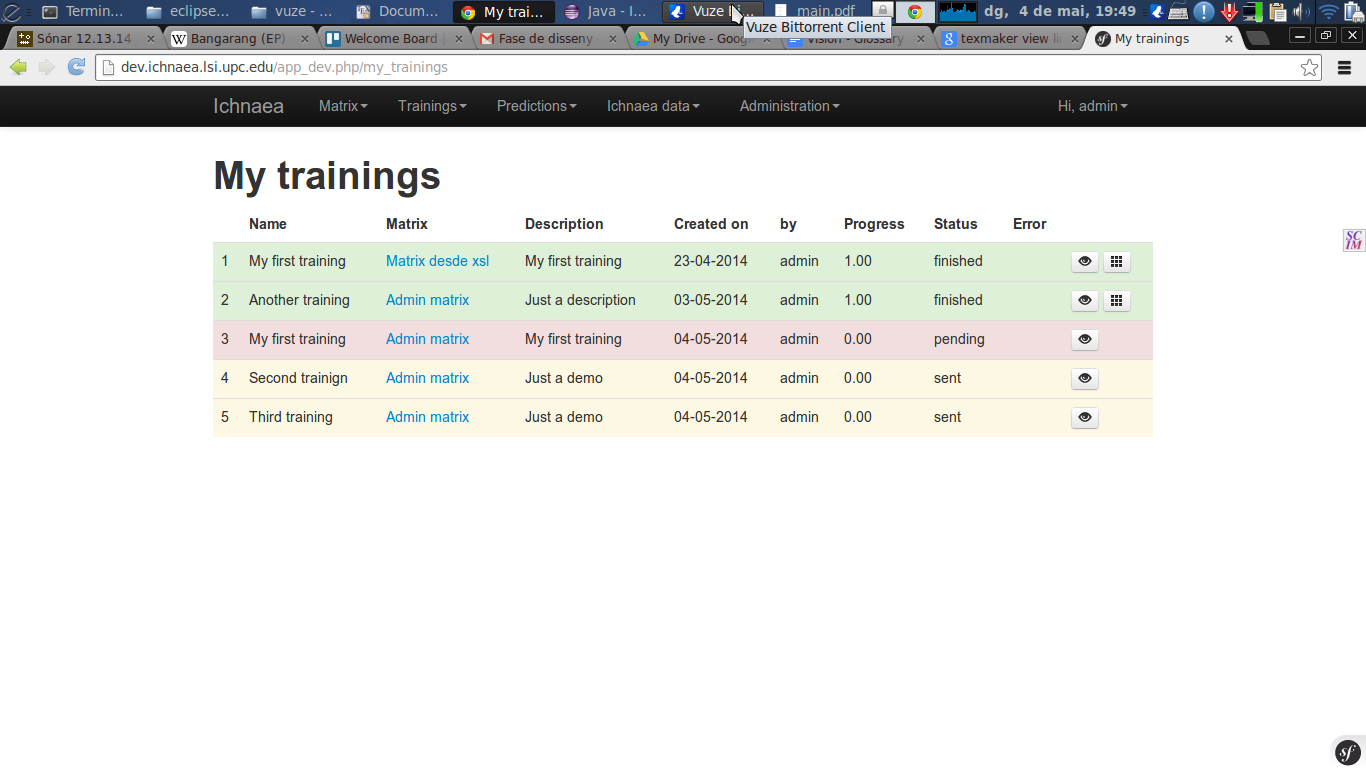
\includegraphics[scale=0.4]{img/userguide/my_trainings.png}
  \caption{Els meus entrenaments}
  \label{fig:my_trainings}
\end{figure}
On:
\begin{itemize}
\item Nom del entrenament.
\item Nom de la matriu entrenada com a enllaç per veure la matriu.
\item Descripci\'{o} del entrenament.
\item Origen: Paràmetre de creació seleccionat per l'entrenament. Actualment solament es guarda el valor pero Ichnaea no esta desenvolupat encara per executar un entrenament amb aquest paràmetre.
\item Data de creaci\'{o} de l'entrenament.
\item Nom de l'usuari que la creat(que sempre serà l'usuari registrat).
\item Progr\'{e}s: actualment Ichnaea no retorna estat del proces. Solament ens diu si ha acabat o no. Per tant els \'{u}nics valors son 0.00 i 1.00.
\item Status. Els possibles status son ''pending''(no s'ha pogut enviar),''sent''(s'ha enviat a la cua) i ''finished''(finalitzat). 
\item Operacions
 \begin{itemize}
 \item \iconeyeopen \'{e}s per anar a la pantalla de visualització de l'entrenament.
 \end{itemize}
\end{itemize}

\subsection{Les meves prediccions}
\label{subsec:myPrediccions}
Per accedir a les teves prediccions, ves al menu ''Predictions >> My predictions''.
\begin{figure}[h!]
  \centering
  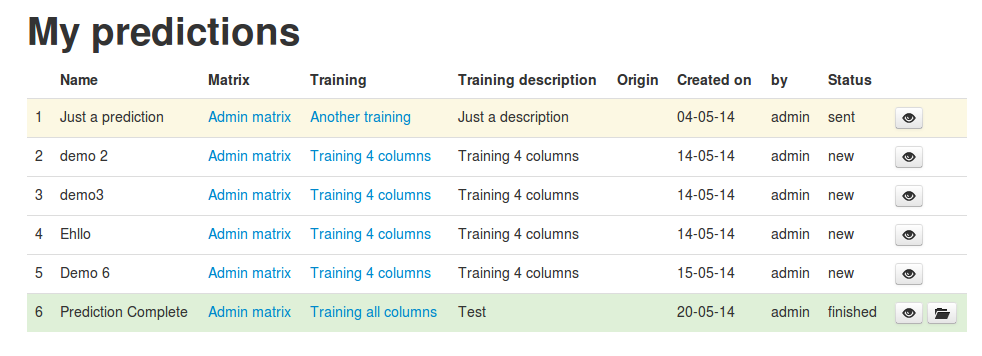
\includegraphics[scale=0.4]{img/userguide/my_predictions.png}
  \caption{Les meves prediccions}
  \label{fig:my_predictions}
\end{figure}
\begin{itemize}
\item Nom de la predicció.
\item Nom de la matriu entrenada com a enllaç per veure la matriu.
\item Nom de l'entrenament com a enllaç per veure quin entrenament s'esta usant per la predicció.
\item Descripció el entrenament que s'esta usant en la predicció.
\item Origen: Paràmetre de creació seleccionat per l'entrenament. Actualment solament es guarda el valor pero Ichnaea no esta desenvolupat encara per executar una entrenament amb aquest paràmetre.
\item Data de creaci\'{o} de la predicció.
\item Nom de l'usuari que la creat(que sempre serà l'usuari registrat).
\item Status. Els possibles status son ''pending''(no s'ha pogut enviar),''sent''(s'ha enviat a la cua), ''finished''(ha finalitzat) i ''new''(s'esta configurant encara la matriu de predicció).
\item Error: en cas que hi hagues algun error en el entrenament desde Ichnaea, sortiria un breu descripcio.(Mirar \ref{subsec:trainingerrorsIchnaea})
\item Operacions
 \begin{itemize}
 \item \iconeyeopen \'{e}s per anar a la pantalla de visualització de l'entrenament.
 \item \iconresults \'{e}s per consultar els resultats.
 \end{itemize}
\end{itemize}

\section{Variables}
\subsection{Veure les variables del sistema}
Desde el menu ''Ichnaea  Data - View Variables'', es poden veure totes les variables del sistema. Amb la icona \iconeyeopen, es pot accedir a la interfície de configuraci\'{o} de la variable seleccionada.

\subsection{Formulari de edici\'{o} d'una variable}
\begin{figure}[h!]
  \centering
  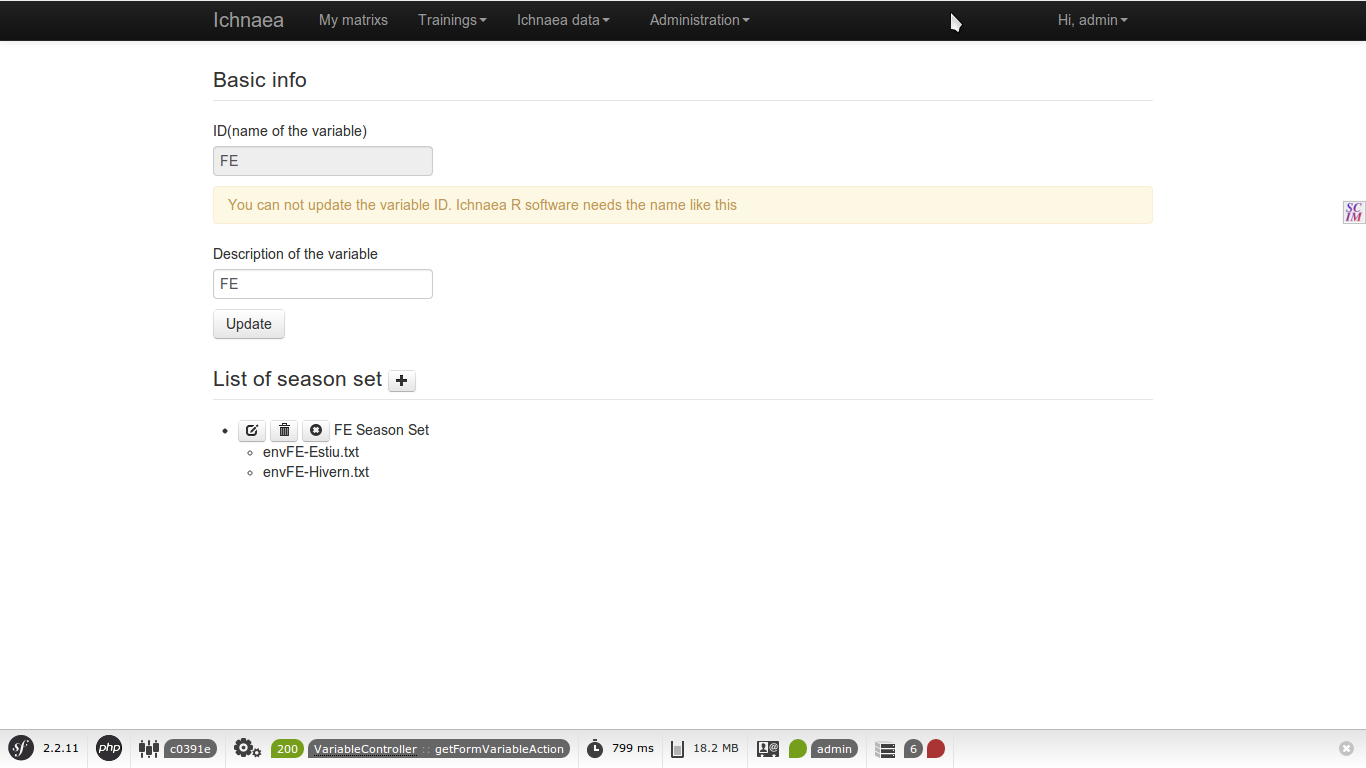
\includegraphics[scale=0.5]{img/userguide/variable_configuration.png}
  \caption{Configuraci\'{o} de variable}
  \label{fig:placement}
\end{figure}
\subsection*{Informació bàsica}
L' ID \'{e}s l'identificador d'Ichnaea i la descripció \'{e}s un camp modificable per descriure la variable.
\subsection{Llistat de conjunts de fitxers: ''season set''}
Son els conjunts de fitxers amb el seus components on:
\begin{itemize}
\item \iconedit per modificar el conjunt de fitxers(nom, components i configuracions).
\item \icontrash per esborrar tot el conjunt i tots el fitxers associats, excepte els compartits.
\item \iconadd per afegir un conjunt nou de fitxers
\end{itemize}

\subsection{Formulari de creació i d'actualització d'un conjunt de fitxers(''Season set'')}
\label{season_set:variable}
\begin{figure}[h!]
  \centering
  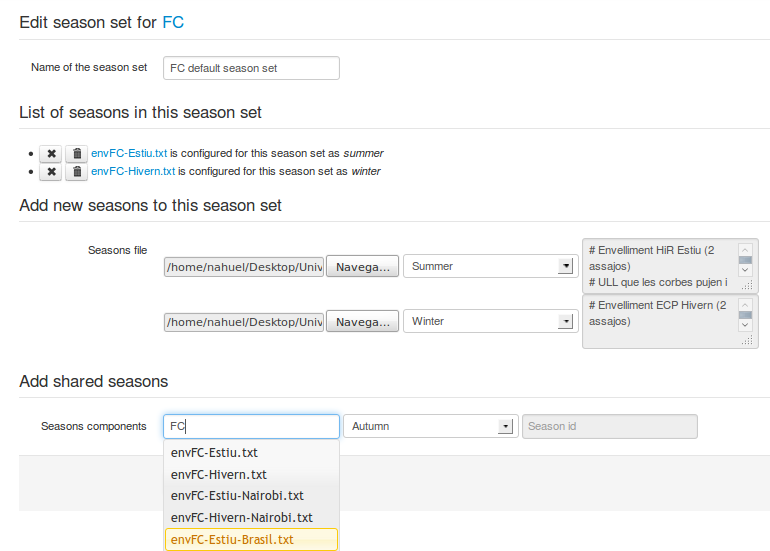
\includegraphics[scale=0.5]{img/userguide/season_set_edition.png}
  \caption{Configuraci\'{o} de conjunts de fitxers d'una variable}
  \label{fig:seasonSetEdition}
\end{figure}

\subsubsection{Afegir nous fitxers a un conjunt de fitxers}
A l'apartat ''Add new seasons to this season set'', \'{e}s pot afegir nous fitxers amb un navegador de fitxer accedint a ''Navega...''. Al selector de temporades es pot configurar el fitxer com estiu, hivern, tardor, primavera o com a tot l'any. El tercer camp \'{e}s un camp especial de tipus ''sols lectura'' per comprovar que el fitxer es carrega be.

\subsubsection{Afegir un fitxer d'una altre variable}
En el cas de que existeixin variables que tinguin envelliments similars, es pot buscar a la secció ''Add shared seasons''. Es un camp de tipus auto-completat que desplega un menú per que l'usuari seleccioni el que busca. Amb el següent selector el pot configurar. L'ultim camp es per comprovar que el fitxer es carrega be.

\subsubsection{Esborrar un fitxer del conjunt de fitxers}
Amb la icona \icontrash pots esborrar el fitxer i el seu contingut d'aquest conjunt de fitxers.\\
Amb la icona \iconremove pots esborrar el fitxer com a component. Per exemple, si has afegit un fitxer compartit, no esborres el fitxer sinó que simplement deixa de estar associat a aquest conjunt de fitxers.

\section{Matrius}
\subsection{Crear una matriu desde un fitxer csv o excel}
\label{sec:create_matrix}
Desde el menu superior ''IchnaeaData - New matrix'', es pot pujat una nova matriu en format csv o Microsoft Excel. El format csv es compatible amb les programaris de ofim\`{a}tica m\'{e}s habituals como Microsoft Excel o Libreoffice.
El format de la matriu \'{e}s important que sigui el següent.
\begin{center}
    \begin{tabular}{ | l | l | l | p{5cm} |}
    \hline
    Cel.la buida & Alias de la columna & .... & ORIGIN & DATE \\ \hline
    Nom de la sample & Valor de la sample  & .... & Origen de la sample \\ \hline
    S01-10-20        & 0,000145            & .... & Human \\ \hline
    \hline
    \end{tabular}
\end{center}
On:
\begin{itemize}
\item Alias de la columna: \'{e}s un nom qualsevol per identificar la columna. Si el sistema cont\'{e} una variable amb el mateix nom, autom\`{a}ticament li assignar aquesta variable amb una ''season set'' per defecte. Si l'alias de variable definit al full de c\`{a}lcul \'{e}s el mateix que el d'una variable del sistema, s'assigna a la variable i li assignar un conjunt de fitxers per defecte.
\item Valor de la sample: \'{e}s el valor de la mostra per la columna(variable)
\item Nom de la sample: \'{e}s un identificador de la mostra. La aplicaci\'{o} mapeja el contingut de subcadenas amb:
\begin{itemize}
\item PL - POULTRY
\item HM - HUMAN
\item PG - PIG
\item CW - COW
\end{itemize}
\item Origen de la mostra: \'{e}s una cadena de caràcters que especifica l'origen de la mostra. Solament es distingir\'{a} si a les capçaleres a la ultima columna s'especifica la paraula ORIGIN. Es OPCIONAL. 
\item Data de la mostra: \'{e}s una data de calendari. Amb el format DIA(DD)/MES(MM)/ANY(YYYY). Per exemple 01/12/2014. Es OPCIONAL. 
\end{itemize}
Important: l'ordre de les columnes \'{e}s important. Si volem deixar la columna origen buida però posar dates, s'ha d'especificar igualment la columna i deixar-la buida. I l'origen de la mostra es resoldra amb el mapejat abans explicat.
En la pantalla, es pot seleccionar un fitxer csv i pujar'ho. Seguidament, es podr\`{a} establir la relaci\'{o} de la variable real de la columna i quin conjunt de fitxers per defecte usa. Mirar \ref{sec:configure_matrix}.

\section{Configurar una matriu}
\label{sec:configure_matrix}
Per accedir a configurar una matriu, has d'anar a la teva pantalla de inici(mirar \ref{sec:home}). 
Desde la interficie de configuraci\'{o} es pot configurar:
\begin{itemize}
\item Donar un alias a la columna
\item Associar una columna a una variable
\item Seleccionar un conjunt de fitxers de la variable
\item Donar nom a una mostra
\item Donar una data a una mostra
\item Donar un origen a un mostra
\item Visualitzar missatges de validacions i notificacions
\item Donar acc\'{e}s als usuaris per que puguin crear trainings.
\end{itemize}
\begin{figure}[h!]
  \centering
  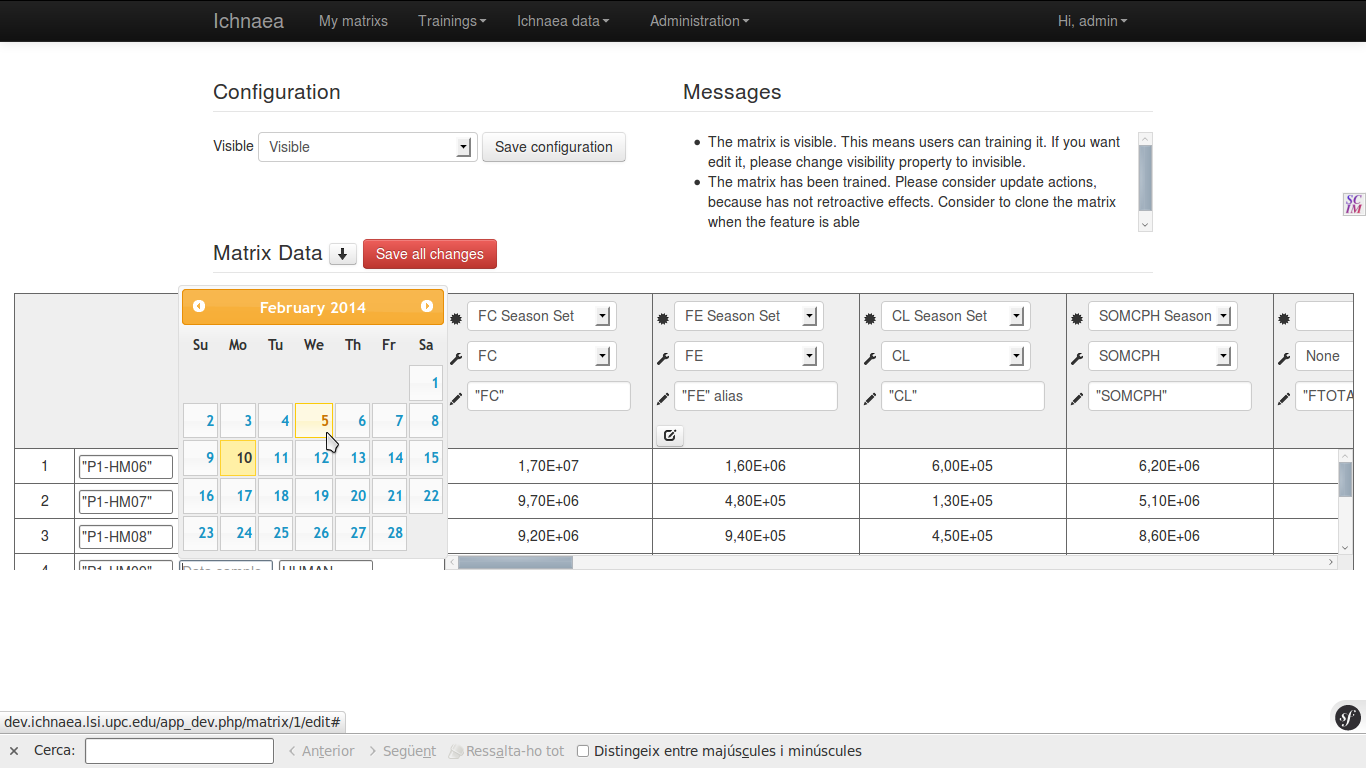
\includegraphics[scale=0.2]{img/userguide/matrix_configure.png}
  \caption{Interficie de configuraci\'{o} de matrius}
  \label{fig:configure_matrix}
\end{figure}

\subsection{Alies de una columna} 
A la secci\'{o} de les capçaleres, a la icona del llapis, es pot especificar un alies a la columna. Si es prem "Enter" o es canvia el focus, s'activa el bot\'{o} de salvaguardat.

\subsection{Especificar en una columna una variable i un conjunt de fitxers}
A la secci\'{o} de les capçaleres, a la icona de la clau anglesa, es pot seleccionar la variable del sistema. Autom\'{a}ticament, a la llista de dalt, es carrega la llista de "Seasons Set". Quan es selecciona un dels dos llistats, s'activa el bot\'{o} de salvaguardat. No \'{e}s obligatori donar-li una variable i una "Season Set".

\subsection{Cambiar la visualitzaci\'{o}}
A la secci\'{o} de configuraci\'{o}, es pot cambiar la visibilitat. Si la matriu \'{e}s invisible, els usuaris no poden crear ''trainings''. Per guardar els canvis, s'ha de pitjar el but\'{o} "Save configuration".

\subsection{Visualitzar missatges}
Existeixen diverses restriccions i missatges:
\begin{itemize}
\item Notificaci\'{o} de visibilitat: una matriu visible es entrenable. 
\item Notificaci\'{o} de matriu amb trainings creats. Una modificaci\'{o} crea una incoherencia amb aquests trainings ja que no ser\'{a} la mateixa matriu.
\item Notificaci\'{o} d'origens. Les mostres necessiten obligatoriament uns origins.
\end{itemize}

\subsection{Actualitzar una dada d'una fila i d'una columna}
Es poden actualitzar les dades d'una mostra i d'una 

\section{Clonar una matriu}
\label{sec:clone_matrix}
Desde el menu ''Ichnaea Data - View Matrix'', podem accedir al llistat de variables del sistema. Amb la icona etiquetada com "Clone the matrix", podem clonar una matriu sencera configurada. No es copien els trainings.
\begin{figure}[h!]
  \centering
  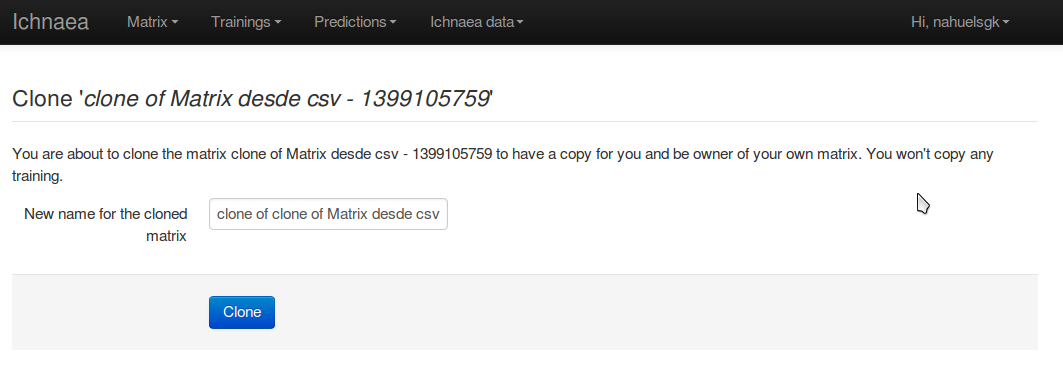
\includegraphics[scale=0.2]{img/userguide/clone_matrix.png}
  \caption{Llistat de matrius}
  \label{fig:placement}
\end{figure}
Fent click a la icona de reload, anem al formulari que suggereix un nom per identificar-la.
\begin{figure}[h!]
  \centering
  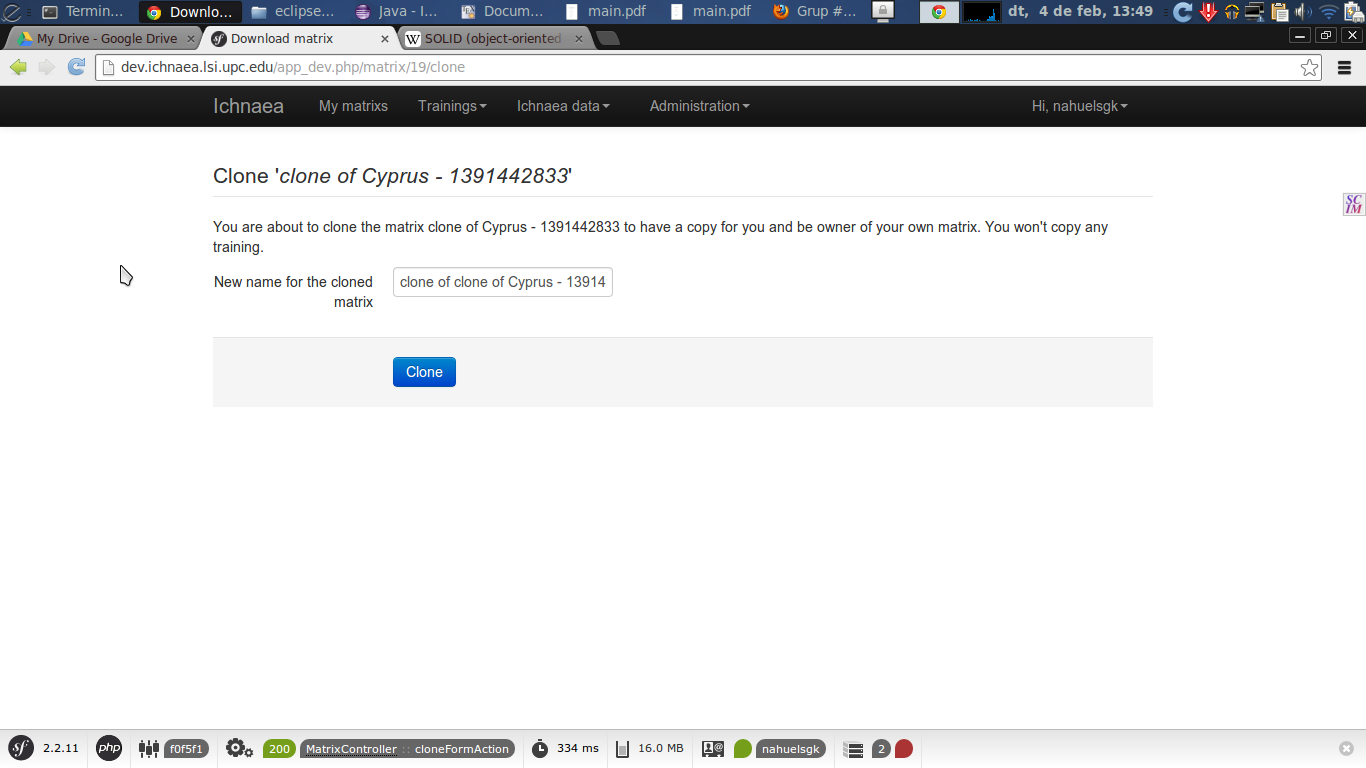
\includegraphics[scale=0.2]{img/userguide/clone_matrix-2.png}
  \caption{Llistat de matrius}
  \label{fig:placement}
\end{figure}
Acceptant, es clona la matriu i anem a la interficie de configuraci\´{o}. Mirar \ref{sec:configure_matrix}.

\section{Crear un training d'una matriu}
Per crear un training s'ha de accedir al menu superior ''Trainings - Create a training''. Desde el llistat de matrius del sistema, amb la icona ICONROAD, es pot accedir al formulari de creaci\'{o} de trainings.
\begin{figure}[h!]
  \centering
  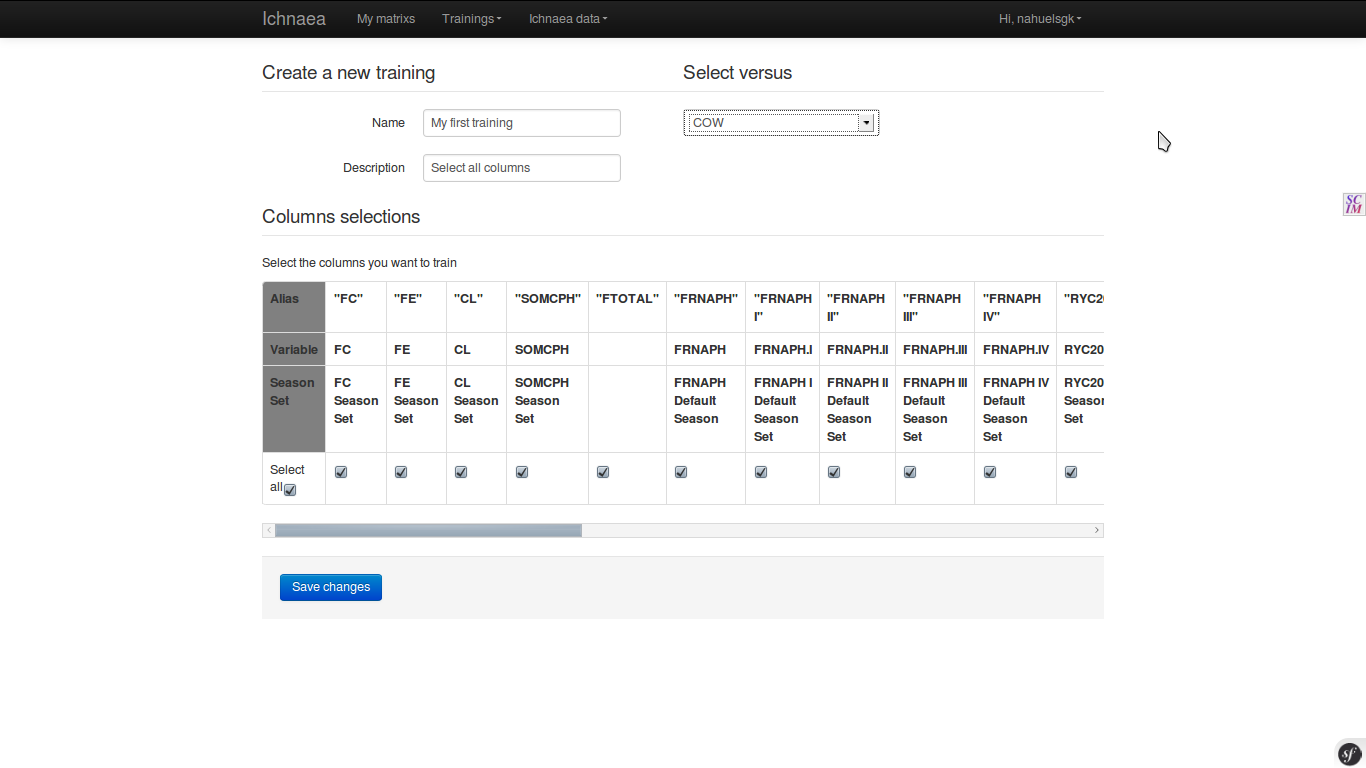
\includegraphics[scale=0.2]{img/userguide/training_create.png}
  \caption{Llistat de matrius}
  \label{fig:placement}
\end{figure}
\begin{itemize}
\item Part esquerra superior: El training cont\'{e} un nom i una descripci\'{o}. Es poden seleccionar quines columnes vols entrenar de la matriu. 
\item Part dreta superior: Desplegable per seleccionar un dels origens disponibles.  El origen-versus, es un llistat de la variable origen de la matriu. Si es selecciona el valor "All versus all", el training ser\'{a} tots contra tots. Si \'{e}s selecciona un origen concret, el training es far\`{a} aquest origen contra els altres. Actualment Ichnaea no suporta aquesta part per\'{o} en el futur est\`{a} planificat que ho far\`{a}.
\item Selecci\'{o} de columnes. Selecci\'{o} de columnes que vols entrenar.
\end{itemize}

Si la creaci\´{o} \´e{s} correcte, les dades s'enviaran a la cua de procesos i la aplicaci\´{o} es redirigir\´{a} la pantalla de visualitzaci\´{o} de trainings.

\subsection{Simular un training de la matriu Cyprus}
Actualment la aplicaci\'{o} Ichnaea i el sistema de cues no esta implantat. Tenim la opci\'{o} de tenir una matriu entrenada en un altre plataforma per poder fer proves amb les interficies de prediccions. Pendent d'implementaci\'{o}.

\section{Visualitzar un training}
Desde la casa de l'usuari(mirar \ref{sec:home}), es pot veure els teus trainings i en quin estadi es troben. Amb la icona "ull", pots accedir a visualitzar la informaci\´{o} del training.

\section{Problemes de Ichnaea}
\label{sec:ichnaeaErrors}
\subsection{Error en els entrenaments}
\begin{figure}[h!]
  \centering
  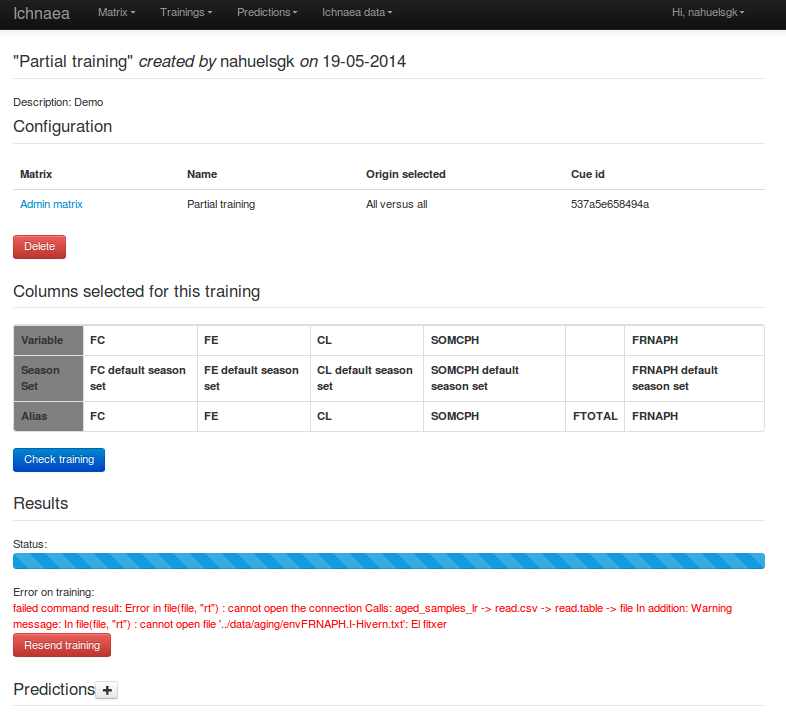
\includegraphics[scale=0.2]{img/userguide/view_training_pending.png}
  \caption{Training que es pot enviar a la cua}
  \label{fig:placement}
\end{figure}

Actualment Ichnaea Software i el sistema de cues no esta implantat. Per defecte, la creaci\'{o} donar\'{a} error. Per tant, es pot utilitzar la simulaci\'{o} de trainings.
A banda d'aix\'{o}, tenim predifinits un conjunt de situacions que a continuaci\'{o} descrivim.

\section{Crear una matriu de predicci\'{o}}
Desde la casa de l'usuari, es pot veure els teus trainings i en quin estadi es troben. Amb la icona "Quadradets"

\section{Crear una predicci\'{o}}
Desde la casa de l'usuari(mirar \ref{sec:home}) es pot crear una predicci\'{o} d'un training. Seleccionant la icona ''quadricules'' de un trainig correcte(en color verd), es pot crear un matriu de predicci\'{o}.

\begin{figure}[h!]
  \centering
  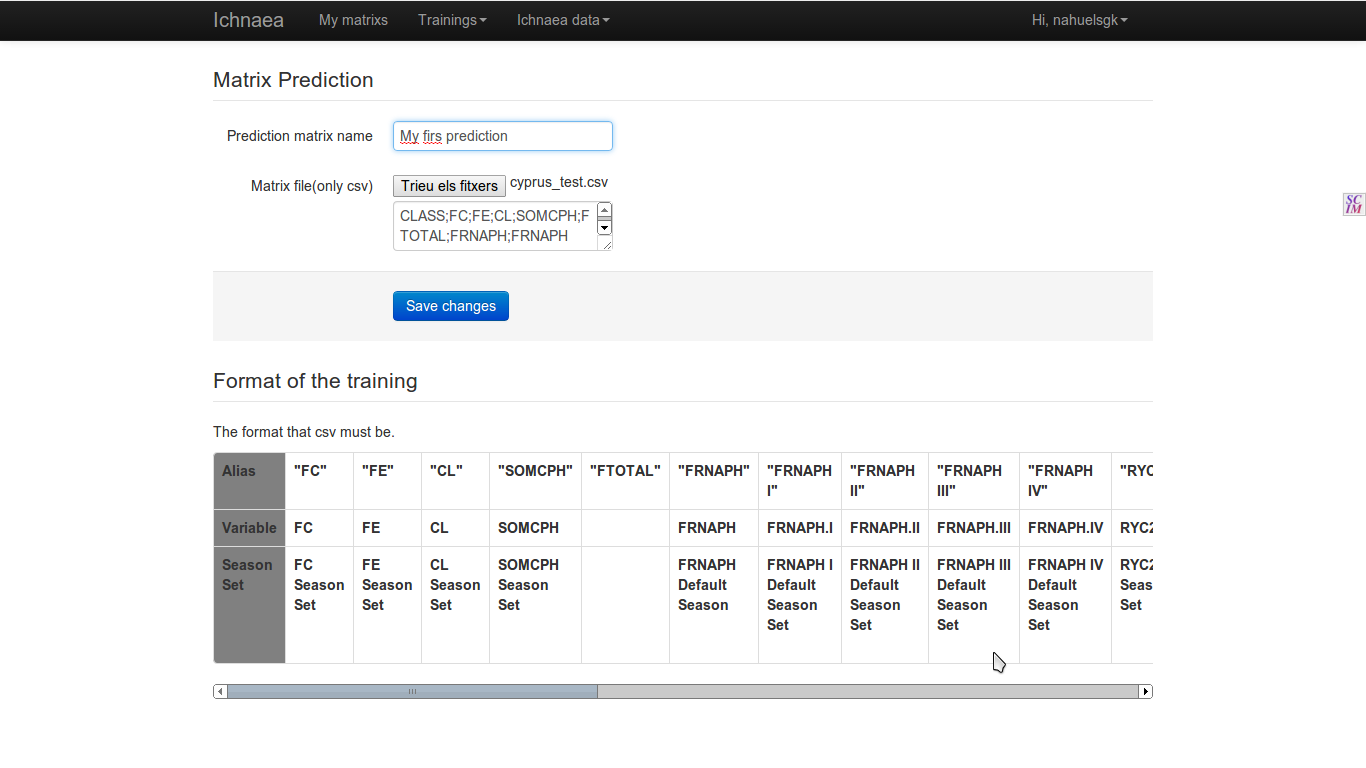
\includegraphics[scale=0.2]{img/userguide/prediction_create.png}
  \caption{Exemple de creaci\'{o} de predicci\'{o}}
  \label{fig:placement}
\end{figure}

A part superior \'{e}s pot seleccionar un fitxer per pujar la matriu per predir. A la part inferior es pot veure les columnes que el training t\'{e} seleccionades. La matrius en format csv ha de tenir el format indicat per la part inferior. En breu es podr\'{a} descarregar una template per tenir el template i poder simplement omplir els valors:
\begin{center}
    \begin{tabular}{ | l | l | l | p{5cm} |}
    \hline
    Cel.la buida & Alias de la columna & .... & ORIGIN \\ \hline
    Nom de la sample & Valor de la sample  & .... & Origen de la sample \\ \hline
    S01-10-20        & 0,000145            & .... & Human \\ \hline
    \hline
    \end{tabular}
\end{center}
Seguidament es pot visualitzar

\section{Actualitzar una matriu de predicci\'{o}}

\section{Llistar les meves prediccions}
Desde el menu superior "Prediction - My predictions" pots llistar les teves prediccions.

\section{Visualitzar una matriu de predicci\'{o}}

\subsection{Actualitzar una matriu de predicci\'{o}}

\subsection{Executar una predicci\'{o} de una matriu de predicci\'{o}}


